\documentclass[border=5pt]{standalone}
\usepackage{pgfplots}
\pgfplotsset{compat=1.18}
\usepackage{siunitx}
\usepackage{tikz}
\usetikzlibrary{calc}

\definecolor{v1Color}{RGB}{31,119,180}  % Blue for v1
\definecolor{v2Color}{RGB}{255,127,14}   % Orange for v2

\begin{document}
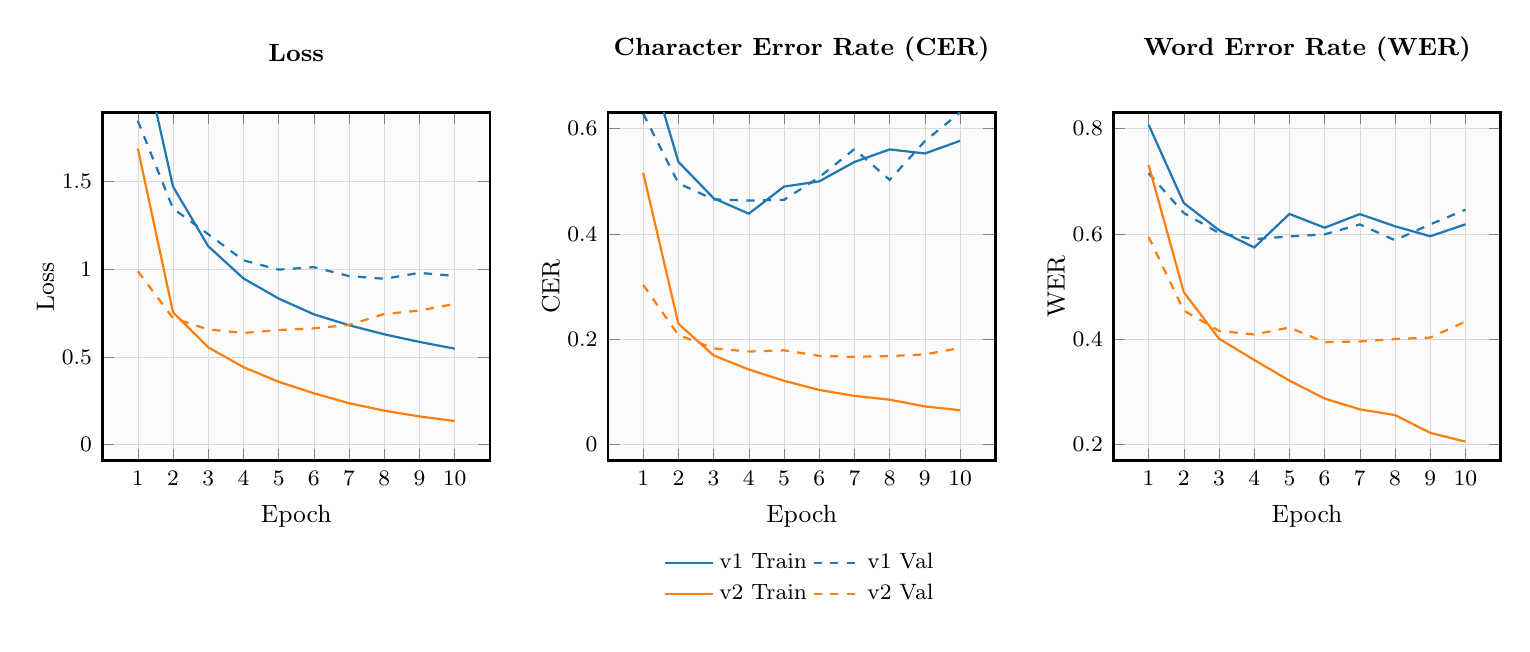
\begin{tikzpicture}[remember picture]

    % Graph 1: Loss
    \begin{axis}[
        name=plot1,
        width=6.5cm,
        height=6cm,
        xlabel={Epoch},
        ylabel={Loss},
        ylabel style={yshift=-0.15cm},
        xmin=0.5, xmax=10.5,
        ymin=0, ymax=1.8,
        xtick={1,2,3,4,5,6,7,8,9,10},
        grid=both,
        grid style={line width=.1pt, draw=gray!10},
        major grid style={line width=.2pt,draw=gray!30},
        title={Loss},
        axis background/.style={fill=gray!3},
        title style={yshift=3mm, font=\small\bfseries},
        label style={font=\small},
        tick label style={font=\footnotesize},
        line width=1pt,
        enlarge x limits=0.05,
        enlarge y limits=0.05,
        every axis plot/.append style={no markers},
        legend to name=commonlegend,
        legend columns=2,
        legend style={draw=none, fill=none, font=\footnotesize}
    ]
        % v1 Train (first 10 epochs)
        \addplot[color=v1Color, thick] coordinates {
            (1, 2.3660) (2, 1.4690) (3, 1.1299) (4, 0.9464) (5, 0.8319)
            (6, 0.7422) (7, 0.6801) (8, 0.6283) (9, 0.5850) (10, 0.5467)
        };
        
        % v1 Validation (first 10 epochs)
        \addplot[color=v1Color, thick, dashed] coordinates {
            (1, 1.8435) (2, 1.3443) (3, 1.1983) (4, 1.0496) (5, 0.9964)
            (6, 1.0106) (7, 0.9597) (8, 0.9445) (9, 0.9781) (10, 0.9606)
        };
        
        % v2 Train
        \addplot[color=v2Color, thick] coordinates {
            (1, 1.6864) (2, 0.7533) (3, 0.5544) (4, 0.4414) (5, 0.3582)
            (6, 0.2928) (7, 0.2364) (8, 0.1938) (9, 0.1611) (10, 0.1348)
        };
        
        % v2 Validation
        \addplot[color=v2Color, thick, dashed] coordinates {
            (1, 0.9872) (2, 0.7209) (3, 0.6562) (4, 0.6361) (5, 0.6526)
            (6, 0.6623) (7, 0.6813) (8, 0.7440) (9, 0.7637) (10, 0.8013)
        };
        
        \legend{v1 Train, v1 Val, v2 Train, v2 Val}
    \end{axis}
    
    % Graph 2: CER, positioned to the right of plot1
    \begin{axis}[
        name=plot2,
        at={($(plot1.east)+(1.5cm,0)$)},
        anchor=west,
        width=6.5cm,
        height=6cm,
        xlabel={Epoch},
        ylabel={CER},
        ylabel style={yshift=-0.15cm},
        xmin=0.5, xmax=10.5,
        ymin=0, ymax=0.6,
        xtick={1,2,3,4,5,6,7,8,9,10},
        grid=both,
        grid style={line width=.1pt, draw=gray!10},
        major grid style={line width=.2pt,draw=gray!30},
        title={Character Error Rate (CER)},
        axis background/.style={fill=gray!3},
        title style={yshift=3mm, font=\small\bfseries},
        label style={font=\small},
        tick label style={font=\footnotesize},
        line width=1pt,
        enlarge x limits=0.05,
        enlarge y limits=0.05,
        every axis plot/.append style={no markers}
    ]
        % v1 Train (first 10 epochs)
        \addplot[color=v1Color, thick] coordinates {
            (1, 0.7628) (2, 0.5367) (3, 0.4676) (4, 0.4383) (5, 0.4897)
            (6, 0.4996) (7, 0.5364) (8, 0.5602) (9, 0.5525) (10, 0.5765)
        };
        
        % v1 Validation (first 10 epochs)
        \addplot[color=v1Color, thick, dashed] coordinates {
            (1, 0.6280) (2, 0.4960) (3, 0.4654) (4, 0.4633) (5, 0.4646)
            (6, 0.5074) (7, 0.5608) (8, 0.5024) (9, 0.5759) (10, 0.6303)
        };
        
        % v2 Train
        \addplot[color=v2Color, thick] coordinates {
            (1, 0.5158) (2, 0.2296) (3, 0.1693) (4, 0.1427) (5, 0.1213)
            (6, 0.1039) (7, 0.0926) (8, 0.0855) (9, 0.0727) (10, 0.0655)
        };
        
        % v2 Validation
        \addplot[color=v2Color, thick, dashed] coordinates {
            (1, 0.3032) (2, 0.2081) (3, 0.1828) (4, 0.1768) (5, 0.1791)
            (6, 0.1686) (7, 0.1667) (8, 0.1682) (9, 0.1713) (10, 0.1834)
        };
    \end{axis}
    
    % Graph 3: WER, positioned to the right of plot2
    \begin{axis}[
        name=plot3,
        at={($(plot2.east)+(1.5cm,0)$)},
        anchor=west,
        width=6.5cm,
        height=6cm,
        xlabel={Epoch},
        ylabel={WER},
        ylabel style={yshift=-0.15cm},
        xmin=0.5, xmax=10.5,
        ymin=0.2, ymax=0.8,
        xtick={1,2,3,4,5,6,7,8,9,10},
        grid=both,
        grid style={line width=.1pt, draw=gray!10},
        major grid style={line width=.2pt,draw=gray!30},
        title={Word Error Rate (WER)},
        axis background/.style={fill=gray!3},
        title style={yshift=3mm, font=\small\bfseries},
        label style={font=\small},
        tick label style={font=\footnotesize},
        line width=1pt,
        enlarge x limits=0.05,
        enlarge y limits=0.05,
        every axis plot/.append style={no markers}
    ]
        % v1 Train (first 10 epochs)
        \addplot[color=v1Color, thick] coordinates {
            (1, 0.8072) (2, 0.6585) (3, 0.6070) (4, 0.5742) (5, 0.6378)
            (6, 0.6117) (7, 0.6375) (8, 0.6144) (9, 0.5955) (10, 0.6181)
        };
        
        % v1 Validation (first 10 epochs)
        \addplot[color=v1Color, thick, dashed] coordinates {
            (1, 0.7151) (2, 0.6396) (3, 0.6017) (4, 0.5900) (5, 0.5951)
            (6, 0.5991) (7, 0.6179) (8, 0.5879) (9, 0.6181) (10, 0.6458)
        };
        
        % v2 Train
        \addplot[color=v2Color, thick] coordinates {
            (1, 0.7310) (2, 0.4895) (3, 0.4012) (4, 0.3608) (5, 0.3216)
            (6, 0.2876) (7, 0.2671) (8, 0.2563) (9, 0.2225) (10, 0.2058)
        };
        
        % v2 Validation
        \addplot[color=v2Color, thick, dashed] coordinates {
            (1, 0.5945) (2, 0.4546) (3, 0.4160) (4, 0.4091) (5, 0.4223)
            (6, 0.3945) (7, 0.3958) (8, 0.4005) (9, 0.4033) (10, 0.4336)
        };
    \end{axis}

    % Positioning the common legend below all graphs
    \node at ($(plot1.south)!0.5!(plot3.south)+(0,-1.5cm)$) {\pgfplotslegendfromname{commonlegend}};
    
\end{tikzpicture}
\end{document}